%%%%%%%%%%%%%%%%%%%%%%%%%%%%%%%%%%%%%%%%%%%%%%%%%%%%%%%%%%%%%%%%%%%%%%%%%%%%%%%%%%%%%%%
%%%%%%%%%%%%%%%%%%%%%%%%%%%%%%%%%%%%%%%%%%%%%%%%%%%%%%%%%%%%%%%%%%%%%%%%%%%%%%%%%%%%%%%
% 
% This top part of the document is called the 'preamble'.  Modify it with caution!
%
% The real document starts below where it says 'The main document starts here'.

\documentclass[12pt]{article}
\usepackage{graphicx}
\usepackage{float}
\usepackage{amssymb,amsmath,amsthm}
\usepackage[top=1in, bottom=1in, left=1.25in, right=1.25in]{geometry}
\usepackage{fancyhdr}
\usepackage{enumerate}
\usepackage{listings}
% Comment the following line to use TeX's default font of Computer Modern.
\usepackage{times,txfonts}

\newtheoremstyle{homework}% name of the style to be used
  {18pt}% measure of space to leave above the theorem. E.g.: 3pt
  {12pt}% measure of space to leave below the theorem. E.g.: 3pt
  {}% name of font to use in the body of the theorem
  {}% measure of space to indent
  {\bfseries}% name of head font
  {:}% punctuation between head and body
  {2ex}% space after theorem head; " " = normal interword space
  {}% Manually specify head
\theoremstyle{homework} 

% Set up an Exercise environment and a Solution label.
\newtheorem*{exercisecore}{Exercise \@currentlabel}
\newenvironment{exercise}[1]
{\def\@currentlabel{#1}\exercisecore}
{\endexercisecore}

\newcommand{\localhead}[1]{\par\smallskip\noindent\textbf{#1}\nobreak\\}%
\newcommand\solution{\localhead{Solution:}}

%%%%%%%%%%%%%%%%%%%%%%%%%%%%%%%%%%%%%%%%%%%%%%%%%%%%%%%%%%%%%%%%%%%%%%%%
%
% Stuff for getting the name/document date/title across the header
\makeatletter
\RequirePackage{fancyhdr}
\pagestyle{fancy}
\fancyfoot[C]{\ifnum \value{page} > 1\relax\thepage\fi}
\fancyhead[L]{\ifx\@doclabel\@empty\else\@doclabel\fi}
\fancyhead[C]{\ifx\@docdate\@empty\else\@docdate\fi}
\fancyhead[R]{\ifx\@docauthor\@empty\else\@docauthor\fi}
\headheight 15pt

\def\doclabel#1{\gdef\@doclabel{#1}}
\doclabel{Use {\tt\textbackslash doclabel\{MY LABEL\}}.}
\def\docdate#1{\gdef\@docdate{#1}}
\docdate{Use {\tt\textbackslash docdate\{MY DATE\}}.}
\def\docauthor#1{\gdef\@docauthor{#1}}
\docauthor{Use {\tt\textbackslash docauthor\{MY NAME\}}.}
\makeatother

% Shortcuts for blackboard bold number sets (reals, integers, etc.)
\newcommand{\Reals}{\ensuremath{\mathbb R}}
\newcommand{\Nats}{\ensuremath{\mathbb N}}
\newcommand{\Ints}{\ensuremath{\mathbb Z}}
\newcommand{\Rats}{\ensuremath{\mathbb Q}}
\newcommand{\Cplx}{\ensuremath{\mathbb C}}
%% Some equivalents that some people may prefer.
\let\RR\Reals
\let\NN\Nats
\let\II\Ints
\let\CC\Cplx

%%%%%%%%%%%%%%%%%%%%%%%%%%%%%%%%%%%%%%%%%%%%%%%%%%%%%%%%%%%%%%%%%%%%%%%%%%%%%%%%%%%%%%%
%%%%%%%%%%%%%%%%%%%%%%%%%%%%%%%%%%%%%%%%%%%%%%%%%%%%%%%%%%%%%%%%%%%%%%%%%%%%%%%%%%%%%%%
% 
% The main document start here.

% The following commands set up the material that appears in the header.
\doclabel{Stat 300: Homework 13}
\docauthor{Stefano Fochesatto}
\docdate{\today}

\begin{document}

\begin{exercise}{9.24} Damages to grapes from predation is a serious problem for grape growers \dots Consider the 
  following data on time spent on a single visit to the location,\\

  \begin{enumerate}
    \item Calculate the upper confidence bound for the true average time that blackbirds spend on a single visit at the 
    experimental location.\\
    \solution Finding the $t$-value for a 95\% CI with 64 degrees of freedom we get that $t_{(.025, 64)} = 1.671$. Calculating the upper bound of 
    the confidence interval with the given $\bar{x} = 13.4$, $SE = 2.05$,
    \begin{equation*}
      \bar{x} + t_{(.025, 64)}SE = 13.4 + 1.671(2.05) \approx 16.825. 
    \end{equation*}
    \vspace{.25in}


    \item Does it appear that the true average time spent by blackbirds at the experimental location exceeds the true average time birds of This
    type spend at the natural location? Carry out the test of hypothesis.\\
    \solution First we must use the SE and the sample size to compute the sample standard deviation for each location, 
    \begin{equation*}
      s_1 = 2.05(\sqrt{65}) \approx 16.527,
    \end{equation*}
    \begin{equation*}
      s_2 = 1.76(\sqrt{50}) \approx 12.445.
    \end{equation*}
    From the claim made in the problem statement we srt up the hypothesis test as follows,
    \begin{equation*}
      H_0:\mu_1 = \mu_2,
    \end{equation*}
    \begin{equation*}
      H_a:\mu_1 > \mu_2.
    \end{equation*}
    Now we must solve for the test statistic $t$ and it's degrees of freedom $v$,
    \begin{equation*}
      t = \dfrac{\bar{x_1} - \bar{x_2}}{\sqrt{\frac{s_1^2}{n_1} + \frac{s_2^2}{n_2}}} = \dfrac{13.4 - 9.7}{\sqrt{\frac{16.527^2}{65} + \frac{12.445^2}{50}}} = 1.37.
    \end{equation*}
    \begin{equation*}
      v = \dfrac{(SE_1^2 - SE_2^2)^2}{\frac{SE_1^4}{n_1-1}  + \frac{SE_2^4}{n_2 - 1}} = \dfrac{(2.05^2 - 1.76^2)^2}{\frac{2.05^4}{64}  + \frac{1.76^4}{49}} \approx 112. 
    \end{equation*}
    Assuming a significance level of $\alpha = .05$. From our table A.5 we can see that our $P$ is greater that our significance level and therefore we 
    fail to reject the null hypothesis. 
    \vspace{.25in}
  
    \item Estimate the difference between the true average time blackbirds spend at the natural location and the true average time that silvereyes spend at the natural 
    location, and do so in a way that conveys information about reliability and precision.\\
    \solution To proceed we will calculate a 95\% CI for $\bar{x_1} - \bar{x_2}$, where the sample mean refers to the blackbirds and silvereyes respectively. Solving for the degrees
    of freedom of $\bar{x_1} - \bar{x_2}$,
    \begin{equation*}
      v = \dfrac{(SE_1^2 - SE_2^2)^2}{\frac{SE_1^4}{n_1-1}  + \frac{SE_2^4}{n_2 - 1}} = \dfrac{(1.76^2 - 5.06^2)^2}{\frac{1.76^4}{49}  + \frac{5.06^4}{45}} \approx 55. 
    \end{equation*}
    Then using the SE and the sample size to compute the sample standard deviations, 
    \begin{equation*}
      s_1 = 1.76(\sqrt{50}) \approx 12.445,
    \end{equation*}
    \begin{equation*}
      s_2 = 5.06(\sqrt{46}) \approx 34.317.
    \end{equation*}
    Using our table we get that $t_{(.025, 55)} = 2.006$. Finally we can calculate the 95\% CI for the difference of means. 
    \begin{equation*}
      95\%CI = (9.7 - 38.4 \pm 2.009 \sqrt{\frac{12.445^2}{50} +\frac{34.317^2}{46}}) \approx (-10.84, 10.68)
    \end{equation*}
  \end{enumerate}
\end{exercise}
\vspace{.5in}













\begin{exercise}{9.28} As the population ages, there is increasing concern about accident-related injuries to the elderly\dots Does the data suggest
  that true average maximum lean angle for older females is more than 10 degrees smaller than it is for younger females? State and test the relative hypothesis
  at a significance level .10\\

  \solution First we need to compute the sample mean and standard deviation for each set of data.\\
  \textbf{Console:}
  \begin{center}
  \lstinputlisting{YFvOF.txt}
  \end{center}
  Given the problem statement we get the following one sided hypothesis test,
  \begin{equation*}
    H_0:\mu_1 - \mu_2 = 10,
  \end{equation*}
  \begin{equation*}
    H_a:\mu_1 - \mu_2 > 10.
  \end{equation*}
Finally determining the test statistic $t$ and degrees of freedom $df$,\\
\textbf{Console:}
\begin{center}
\lstinputlisting{YFvOF2.txt}
\end{center}
Using $r$ we get a $p-value = 0.0007221$ which is far below our significance level of $.10$ which means that we reject the Null hypothesis
and claim that the true average maximum lean angle for older females is more than 10 degrees smaller than it is for younger females.\\

Consider the qqnorm plot for each data set.\\
\begin{figure}[H]
  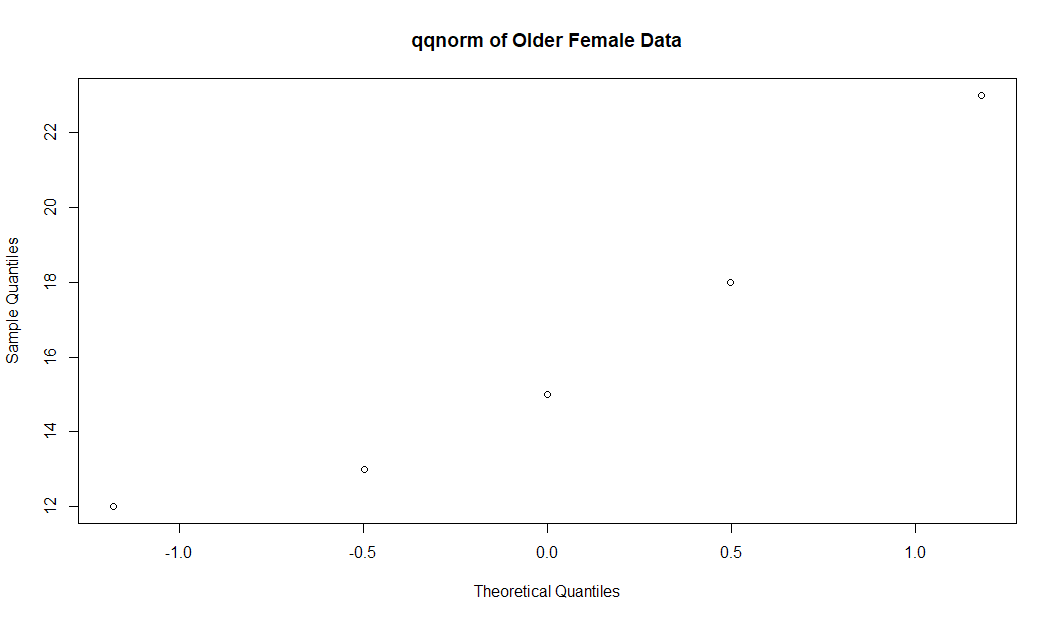
\includegraphics[width = \textwidth]{OF.png}  
  \centering
\end{figure}

\begin{figure}[H]
  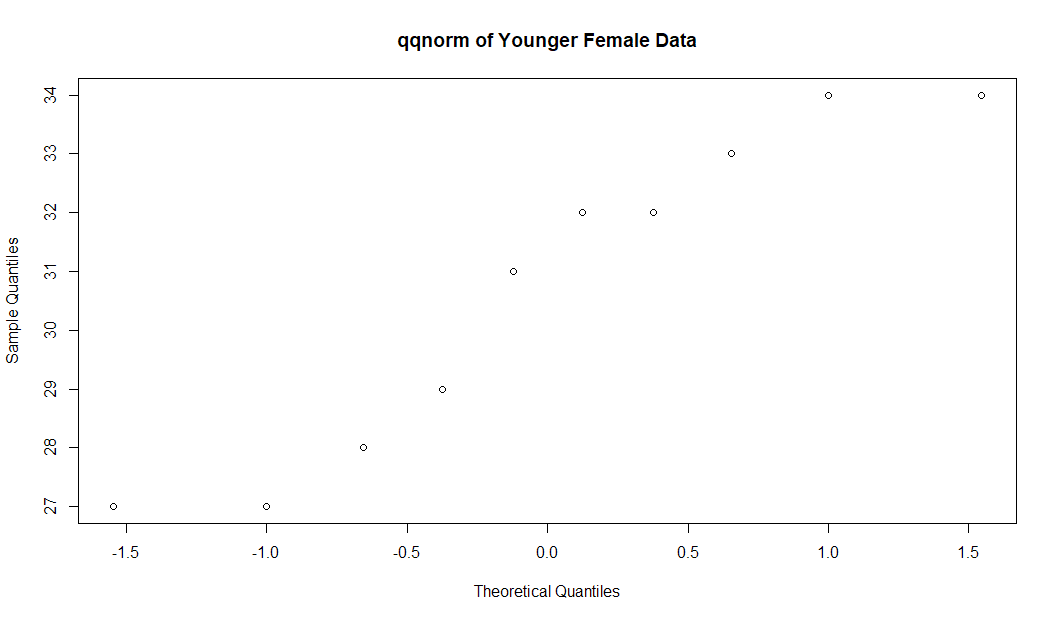
\includegraphics[width = \textwidth]{YF.png}  
  \centering
\end{figure} 
\end{exercise}

Note that with the limited data points we can see the qqnorm plot for the older female data has a slight curve to it. This suggests that 
the data itself is skewed. However with so little data its difficult for me to asses the normality, visually. 
\vspace{.5in}




















\begin{exercise}{9.42}  many freeways have service signs that give information on attractions, camping, lodging, food,
   and gas services prior to off-ramps. These signs typically do not provide information on distance\dots carry out a 
   paired $t$ test to determine whether there was any change in the mean number of crashes before and after the addition of
   distance information on the signs.\\

   \solution From the problem statement we get the following hypothesis test,
   \begin{equation*}
    H_0:\mu_1 - \mu_2 = 0,
  \end{equation*}
  \begin{equation*}
    H_a:\mu_1 - \mu_2 \neq 0.
  \end{equation*}
  Solving for our test statistic $t$ for a paired $t$ test,
  \begin{equation*}
    t = \dfrac{\overline{d}}{s_d/\sqrt{n}} = .72562
  \end{equation*}
  Where $D$ is the pairwise difference between datasets,\\
  \textbf{Console:}
  \begin{center}
  \lstinputlisting{beforevafter.txt}
  \end{center}
  Either using the table or $r$ we get a $p - value \approx .5$. Compared to a significance level of 
  $\alpha = .05$ we get that we fail to reject the Null hypothesis.\\
  Calculating a 95\% CI for $\overline{d}$ by using a $2$- sided critical value of $z_{(.025,5)}$,
  \begin{equation*}
    95\% CI = (5.83 \pm 2.571 \frac{19.69}{\sqrt{6})} = (-14.83,26.49)
  \end{equation*}

\end{exercise}
\vspace{.5in}




















\begin{exercise}{9.50} Recent incidents of food contamination have caused great concern among consumers\dots
  35 of 80 randomly selected Perdue brand broilers tested positively for either campylobacter or salmonella. Whereas
  66 of 80 Tyson brans broilers tested positive. \\
\begin{enumerate}
  \item Does it appear that the true proportion of non-contaminated Perdue broilers differs from that for the 
  Tyson brand? Carry out the hypothesis test using a significance level of $\alpha = .01$\\ 
  \solution From the problem statement we know the following sample proportions, 
  \begin{equation*}
    \hat{p_1} = \dfrac{35}{80}
  \end{equation*} 
  \begin{equation*}
    \hat{p_2} = \dfrac{66}{80}
  \end{equation*} 
  We also know that since they are asking if the true proportions differ, we set up the following Hypothesis test,
  \begin{equation*}
    H_0: p_1 - p_2 = 0,
  \end{equation*}
  \begin{equation*}
    H_a: p_1 - p_2 \neq 0.
  \end{equation*}
  Based on our assumption in the null hypothesis we get that the point estimator for the combined sample proportion is,
  \begin{equation*}
    \hat{p} = \dfrac{35 + 66}{160} = \dfrac{101}{160}
  \end{equation*}
  Solving for our test statistic $z$,
  \begin{equation*}
    z = \dfrac{ \frac{35}{80}   + \frac{66}{80}   }{\sqrt{ \frac{101}{160}\frac{59}{160} (\frac{1}{40})}} \approx -5.08 
  \end{equation*}  
  From our Table A.3 we can clearly see that a test statistic of $z = -5.08$ we get a $p-value$ that is guaranteed to be 
  greater than $\alpha$ and thus there is sufficient evidence eot reject the null hypothesis and claim that 
  the true proportion of non-contaminated Perdue broilers differs from that for the 
  Tyson brand.
  \vspace{.25in}



  \item If the true proportions of non-contaminated chickens form the perdue and tyson brands are $.50$ and $.25$
  respectively, how likely is it that the null hypothesis of equal proportions will be rejected when a $.01$ significance
  level is used and the sample sizes are both 80?\\
  \solution 



\end{enumerate}
\end{exercise}
\vspace{.5in}















\begin{exercise}{12.6} One factor in the development of tennis elbow, a malady that strikes fear in the hearts of all serious tennis players,
  is the impact-induced vibration of the racket-and-arm system at ball contact\dots Consider the scatter plot, and discuss interesting features 
  of the data and scatter plot.\\
  \solution 
  The data looks to have a lot of variation, with two data points in the lower right that would be considered outliers. Outside of those two
  points we can see that there is a negative linear relationship between the racket resonance frequency and sum of peal-to-peak acceleration.\\ 
\end{exercise}
\vspace{.5in}











\begin{exercise}{12.16} Given a scatter plot along with the least squares line of rainfall and runoff volumes for a particular location.\\
  \begin{enumerate}
    \item Does the scatter plot of the data support the use of the simple linear regression model.\\
    \solution The scatter plot definitely supports the use of the simple linear regression model. There is no strong curvature, or even extreme outliers.
    \begin{figure}[H]
      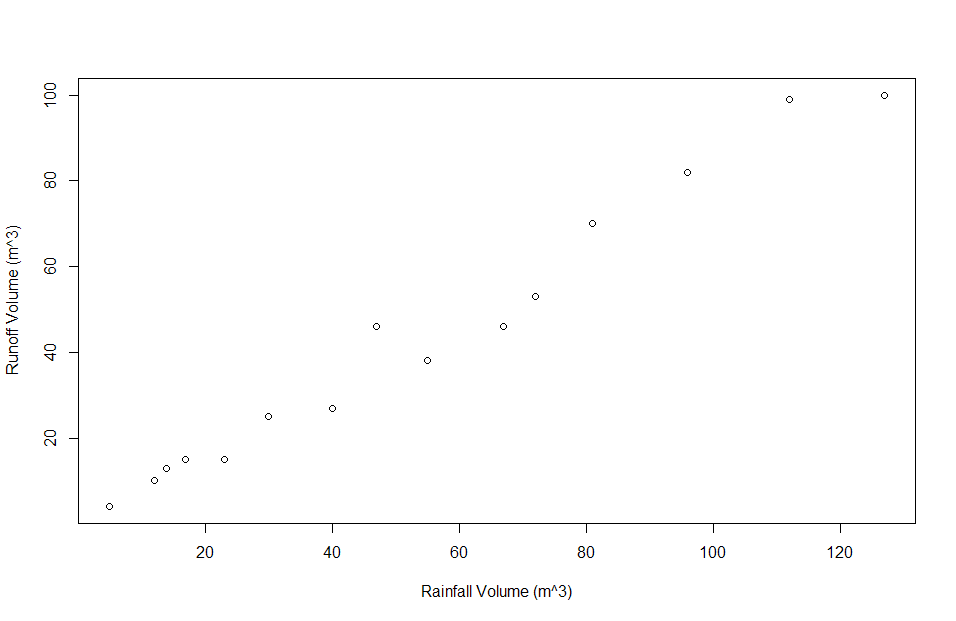
\includegraphics[width = \textwidth]{scatterplot.png}  
      \centering
    \end{figure}
    \vspace{.25in}


    \item Calculate point estimate of the slope and intercept of the population regression line.\\
    \solution Calculating the point estimate for the slope and intercept by using the following least squares solutions,
    \begin{equation*}
      \hat{\beta_1}  = \dfrac{\sum(x_i - \bar{x})(y_i - \bar{y})}{\sum(x_i - \bar{x})^2}.
    \end{equation*}
    \begin{equation*}
      \hat\beta_0  = \bar{y} - \hat\beta_1\bar{x}.
    \end{equation*}
    \textbf{Console:}
    \begin{center}
    \lstinputlisting{simpleregression.txt}
    \end{center}
    Finally we get that our simple linear regression is,
    \begin{equation*}
      f(x) = 0.8269x - 1.1283.
    \end{equation*}
    \begin{figure}[H]
      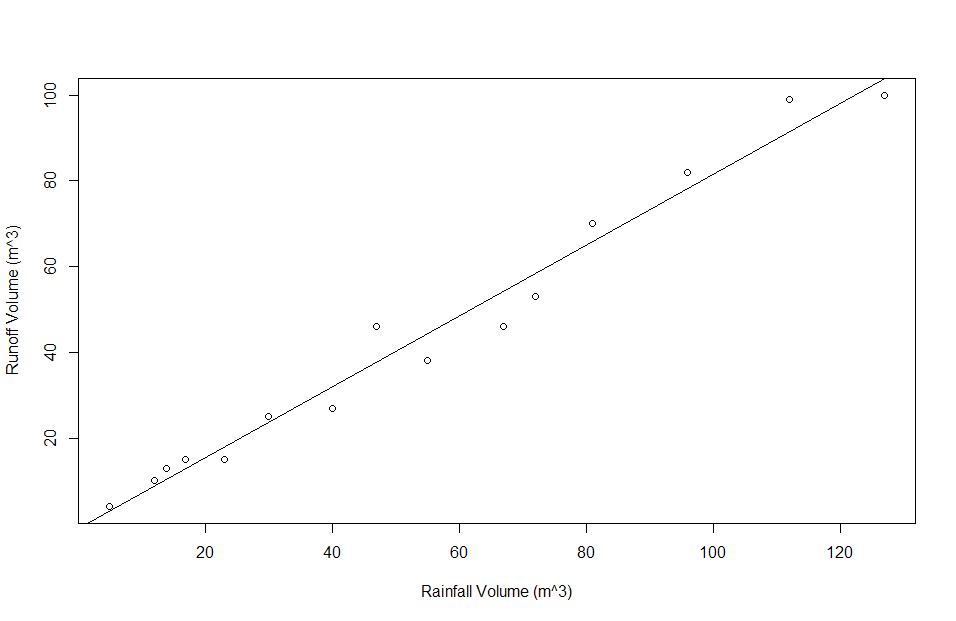
\includegraphics[width = \textwidth]{scatterregression.png}  
      \centering
    \end{figure}
    \vspace{.25in}


    \item Calculate the point estimate of the true average runoff volume when rainfall volume is at 50.\\
    \solution Simply plugging $x = 50$ into our linear regression will yield the desired runoff point estimate.
    \begin{equation*}
      \hat{y} = 0.8269(50) - 1.1283 = 40.2204.
    \end{equation*}

    \item Calculate the point estimate for the standard deviation.\\
    \solution Calculating the point estimate for the standard deviation using our linear regression,
    \begin{equation*}
      \sigma = \sqrt{\dfrac{\sum(y_i - \hat{y_i})^2}{n-2}}.
    \end{equation*}
    \textbf{Console:}
    \begin{center}
    \lstinputlisting{Sigmaregression.txt}
    \end{center}
    \vspace{.25in}

    \item What proportion of the observed variation in runoff volume can be attributed to the simple linear
    regression relationship between runoff and rainfall?\\
    \solution The coefficient of determination is calculated by,
    \begin{equation*}
      r^2 = 1 -  \dfrac{\sum(y_i - \hat{y_i})^2}{\sum(y_i - \overline{y})^2}.
    \end{equation*}
    \textbf{Console:}
    \begin{center}
    \lstinputlisting{coeffdeter.txt}
    \end{center}
    With a $r^2 = 0.9752$ it means that approximately $97.5\%$ of observed variation in runoff volume can be 
    attributed to the simple linear regression relationship between runoff and rainfall.
  \end{enumerate}
\end{exercise}
\vspace{.5in}









\begin{exercise}{12.24} the invasive diatom species\dots Consider the relation between $y =$ colony density, and 
  $x = $rock surface area.\\

  \begin{enumerate}
    \item Fit the simple linear regression model to this data, predict colony density when surface area = 70 and
    when surface area = 71. Calculate the corresponding residuals, how do they compare?\\
    \solution Plugging the data into r and running a similar instruction set to the previous problem we get a linear regression of
    \begin{equation*}
      f(x) = 9.963x - 305.881
    \end{equation*}
    Using our regression to get a point estimate for the density of the colony when $x = 70, 71$,
    \begin{equation*}
      f(70) = 9.963(70) - 305.881 = 391.55,
    \end{equation*}
    \begin{equation*}
      f(x) = 9.963(71) - 305.881  = 401.51.
    \end{equation*}
    Calculating the corresponding residuals,
    \begin{equation*}
      \epsilon_70 =  13 - f(70) = -378.55,
    \end{equation*}
    \begin{equation*}
      \epsilon_71 =  1929 - f(71) = 1527.49.
    \end{equation*}
    Clearly we can see that $\epsilon_71$ is much larger than  $\epsilon_70$. We could see that in general when a linear 
    regression has such large residuals, the coefficient of determination is likely to be very small, making this regression unsuccfull at modeling the relationship 
    between surface area and colony density. 
    \vspace{.25in}

    \item Calculate and interpret the coefficient of determination.\\
    \solution Again calculating the coefficient of determination in r with the same formula described in the previous problem.\\
    \begin{equation*}
      r^2 = 1 -  \dfrac{\sum(y_i - \hat{y_i})^2}{\sum(y_i - \overline{y})^2} \approx 0.12371.
    \end{equation*}
    With a $r^2 = 0.12371$ it means that our linear regression can explain approximately $12.4\%$ of the variation between 
    colony density and rock surface area.
    \vspace{.25in}



    \item Remove the outlier and recalculate the regression. Is it substantially different? What is the impact on $r^2$ and $s$?\\
    \solution After removing the outlying data point and recalculating the linear regression in $r$,
    we get the following function,
    \begin{equation*}
      f(x) = 0.779x + 34.373.
    \end{equation*}
    Note that this function is considerably different from the previous one that we computed. Both the slope and intercept are on the
    order of 10 times smaller than before. Calculating the coefficient of determination $r^2$ and $\sigma$ for both data sets, we get that,
    $r^2 = 0.0238$ and $\sigma =  87.222$ for the new data set, and $\sigma = 5.049835$ for the old data set. We can observe that our new model 
    is even worse than before after removing an extreme outlier.
  \end{enumerate}
\end{exercise}
\vspace{.5in}



\begin{exercise}{12.34} Electro magnetic technologies offer effective nondestructive sensing techniques for determining characteristics of pavement \dots
  Consider that $y =$ dielectric constant and $x =$ air void (\%).\\
\begin{enumerate}
  \item Obtain the equation of the least squares and interpret its slope.\\
  \solution From the given $r$ output we can see that the least squares equation is,
  \begin{equation*}
    f(x) = -.074676x + 4.858691
  \end{equation*}
  Since the slope is negative we know that the lower the air void (\%) the greater the dielectric constant, and on average for an increase of 
  $1\%$ in air void we can expect the dielectric constant to decrease by $.0746$.
  \vspace{.25in}

  \item What proportion of observed variation in dielectric constant can be attributed to the approximate linear relationship between dielectric
  constant and air void.\\
  \solution From the given $r$ output we can see the coefficient of determination is $r^2 = 0.7797$. Therefore  approximately $77.9\%$ of observed variation in dielectric
  constant can be attributed to the simple linear regression relationship between dielectric constant and air void.
  \vspace{.25in}

  \item Does there appear to be a useful linear relationship between dielectric constant and air void? State and test the appropriate hypothesis?
  \solution For this problem we want to use the Model Utility Test, recall the following,
  \begin{equation*}
    H_0 = \beta_1 = 0.
  \end{equation*}
  \begin{equation*}
    H_0 = \beta_1 \neq 0.
  \end{equation*}
Note that when $\beta_1 = 0$ there is no useful linear relationship between dielectric constant and air void. We can see that our test statistic $t$
and $p- value$ are calculated in the given $r$ output,
  \begin{equation*}
  \dfrac{\hat{\beta_1} - 0}{s_{\hat{\beta_1}}} = \dfrac{-0.074676}{0.009923} = -7.526,
  \end{equation*}
  \begin{equation*}
    p = 1.21e-06.
  \end{equation*}
  With such an incredibly small $p - value$ we reject the null hypothesis and therefore it must be the case that there is a significant linear relationship between dielectric constant and air void.
  \vspace{.25in}

    \item Suppose it had previously been believed that when air void increased by 1 percent the associated true average change in dielectric constant would be at least 
    -.05. Does the sample data contradict this belief? Carry out a test of hypothesis with a significance level of $.01$\\
    \solution From the problem statement we set, $\beta_{10} = -.05$ and consider the following hypothesis test,
    \begin{equation*}
      H_0 = \beta_1 = \beta_{10},
    \end{equation*}
    \begin{equation*}
      H_0 = \beta_1 \neq  \beta_{10}.
    \end{equation*}
    Calculating our $t$ statistic using $\hat{\beta_1}$ and $s_{\hat{\beta_1}}$ from the given $r$ output. 
    \begin{equation*}
      \dfrac{\hat{\beta_1} - \beta_{10}}{s_{\hat{\beta_1}}} = \dfrac{-0.074676 - (-.05)}{0.009923} = -.249,
    \end{equation*}
    Using our $r$ calculate a $p- value = 0.8065$ on $16$ degrees of freedom. Since our $p-value$ is considerably larger that our significance level 
    we cannot reject our null and therefore the sample data does not contradict the belief.
\end{enumerate}

\end{exercise}
\vspace{.5in}



\begin{exercise}{12.46} Astringency is the quality in a wine that makes the wine drinker's mouth feel slightly rough, dry, and puckery\dots
  \begin{enumerate}
    \item Fit the simple linear regression model to this data,
    Then determine the proportion of observed variation in astringency that can
    be attributed to the model relationship between 
    astringency and tannin concentration.\\
    \solution From the given summary quantities amd the fact that $\overline{x} = \frac{19.404}{32}$ and $\overline{y} = \frac{-.542}{32}$ and  we can quickly calculate the slope and intercept of linear regression,
    \begin{equation*}
      \hat{\beta_1} = \dfrac{S_{xy}}{S_{xx}} = 2.585,
    \end{equation*}
    \begin{equation*}
      \hat{\beta_0} = \overline{y} - 2.585\overline{x}  = -1.585.
    \end{equation*}
    Thus the function for our linear regression is,
    \begin{equation*}
      f(x) = 2.585x-1.585.
    \end{equation*}
    To solve for the coefficient of determination we must first solve for, Error sum of squares and total sum of squares. By the definition and
    the linearity of sums we reduce to the following formulas,
    \begin{equation*}
      SSE = S_{yy} - \hat{\beta_1}S_{x,y} = 1.9243.
    \end{equation*}  
    \begin{equation*}
      SST = S_{yy} = 11.8263.
    \end{equation*}  
    Finally computing $r^2$,
    \begin{equation*}
      r^2 = 1 - \dfrac{1.9243}{11.8263} \approx .84.
    \end{equation*}
    Thus $84\%$ of the proportion of observed variation in astringency that can
    be attributed to the model relationship between 
    astringency and tannin concentration.
    \vspace{.25in}



    \item Calculate and interpret a confidence interval for the slope of the true regression line.\\
    \solution In order to calculate a $95\%$ CI we must first calculate the point estimate $s_{\hat{\beta_1}}$. Recall that,
    
    \begin{equation*}
      s_{\hat{\beta_1}} = \dfrac{s}{\sqrt{S_{xx}}}.
    \end{equation*}
    
    Also note that the estimate $s$ of standard deviation for $\sigma$,\
    \begin{equation*}
      s = \sqrt{\dfrac{SSE}{n-1}}.
    \end{equation*}
    
    Using our given data we can calculate $s_{\hat{\beta_1}}$,
    \begin{equation*}
      s_{\hat{\beta_1}} = \dfrac{1}{\sqrt{S_{xx}}}\sqrt{\dfrac{SSE}{n-1}} = 0.204664.
    \end{equation*}
    
    Note that the critical value $t_{.025, 30} = 2.042$. Finally calculating our $95\% CI$,
    \begin{equation*}
      95\% CI = (2.585 \pm 2.042(0.204664)) \approx (2.16, 3.01).
    \end{equation*}

    Interestingly even at $95\%$ we are getting a relatively large interval, likely because our sample standard deviation is still relatively large.
  
  
  
  \end{enumerate}
\end{exercise}
\vspace{.5in}




\end{document}